\documentclass{IEEEtran}
%
%\smartqed  % flush right qed marks, e.g. at end of proof
%
\usepackage{graphicx}
%\usepackage{array}
%\usepackage{cite}
%\usepackage[numbers]{natbib}%use numbered citations
%\usepackage{subfigure}
%\usepackage{amsmath}
%\usepackage[indent,bf]{caption2}
%\usepackage{rotating}
%\usepackage{setspace}
%\usepackage{longtable}
%\usepackage{mathrsfs}
%\usepackage{algorithm}
%\usepackage{algpseudocode}


\usepackage{url}
\usepackage{subfigure}

\begin{document}

% first the title is needed
\title{A Distributed Wiki System Based on Peer-to-peer File Sharing Principles}

% the name(s) of the author(s) follow(s) next
%
%


\author{\IEEEauthorblockN{Alexander Craig, Alan Davoust and Babak Esfandiari}

\IEEEauthorblockA{Department of Systems and Computer Engineering\\
Carleton University\\
Ottawa, Canada\\
aaecraig@connect.carleton.ca, adavoust@sce.carleton.ca, babak@sce.carleton.ca}
}
%
%\authorrunning{Towards Semantically Enhanced P2P File-Sharing}
% (feature abused for this document to repeat the title also on left hand pages)

% the affiliations are given next; don't give your e-mail address
% unless you accept that it will be published
%\institute{Department of Systems and Computer Engineering \\
%Carleton University \\
%1125 Colonel By Drive \\
%Ottawa, Ontario, Canada \\
%babak@sce.carleton.ca\\
%adavoust@sce.carleton.ca}
%
%
%
%\IEEEpeerreviewmaketitle
\maketitle

\begin{abstract}
In peer-to-peer (P2P) file-sharing networks, each peer maintains its own repository, publishing files, downloading files from others, and making its own files available for download. We present P2Pedia, a distributed wiki system applying these principles to collaborative edition of documents: contributors may maintain their own version of each document, while accessing and reusing the contributions of others. This collaboration model, by allowing for multiple versions of a document, generates a different type of versioning hierarchy, and changes the semantics of wikilinks. We describe the versioning and wikilinks relationships in terms of more abstract document relationships, present trust indicators to help choose among multiple versions of a document and describe a general approach to answering complex queries over the graph of document induced by the versioning and wikilinks relationships. Finally, we present the design and implementation of P2Pedia, and propose some scenarios where our proposed collaboration model is most appropriate.
\end{abstract}

\begin{IEEEkeywords}
wiki; peer-to-peer; graph queries; trust

\end{IEEEkeywords}

%=====================================================================================================
\section{Introduction}
Wikis were first created by Ward Cunningham as an easy way to edit and maintain web pages directly through the browser, and have become the embodiment of collaborative work on Internet.

In Wikipedia, the coordinated efforts of the web community were leveraged to create a mammoth encyclopedia, which currently contains several million articles in dozens of languages. The usefulness of Wikipedia is obvious from its massive use as an information source, and its factual accuracy has been found to be comparable with that of a traditional encyclopedia \cite{NatureWikipedia}. 

However, critics of Wikipedia disagree with this assessment. Their argument is that since anybody, no matter their qualifications, can edit an article, then those editors are likely to introduce errors and misinformation in Wikipedia. In other words, the problem is that all editors cannot be \emph{trusted}. Traditional encyclopedias, and some recent alternative internet encyclopedias, such as Citizendium \footnote{http://www.citizendium.org/} and ScholarPedia\footnote{http://www.scholarpedia.org/}, address this problem by having only trusted experts edit their content.

The Wikipedia answer would be that the solution to the problem lies precisely in its cause: since anybody can edit articles, factual errors or vandalism are quickly identified and fixed. The underlying rationale is that the editors as a group ultimately reach a consensus, either naturally or following an arbitration process, and that this consensus can be trusted. 

However, a consensus can't always be reached. In Wikipedia, aticles on controversial topics often need to be protected from repeated editing by opposing factions (``edit wars"). Although this choice to accomodate a single viewpoint in Wikipedia may be defendable, this raises a more general question: should collaborative editing always lead to a single, authoritative version of each document? 

To the best of our knowledge, all Wiki systems promote this collaboration model. We explore here a different model, inspired by the principles of Peer-to-peer (P2P) file-sharing: users may maintain different versions of a document, by copying and editing their preferred versions, among those available. 

This collaboration model would solve some of the problems of Wikipedia, described above. Another scenario where this collaboration model to some extent already exists, is the case of learning material, in school or university. Instructors often prepare their teaching material by reusing and adapting material from various sources, and in turn make their own material available to others. Their work can be described as collaborative, without leading to the development of a single, authoritative version. In this sense, we argue that a Wiki system following the same collaboration principles would be a very useful tool, for this scenario and others.

In this paper, we describe a Wiki system built on top of a peer-to-peer (P2P) network, and which supports this collaboration model. Different versions of any article may exist in the network, and user queries return all the relevant versions, from which users must then choose their preferred version to download. The trust problem raised earlier remains relevant: instead of the system implicitly deciding which version of the document should be adopted (the latest version in the case of traditional Wikis), user may establish individual trust relationships, and use these as a basis to choose contributions from the available versions. In addition, this model generates a non-trivial versioning process. In the traditional Wiki collaboration model, there is a linear sequence of versions; in this case there is a tree, or even a lattice of versions, that is important to present to the user. 

Our work makes the following contributions. First, we demonstrate the application of P2P file-sharing principles to collaborative edition by means of a wiki system. Secondly, we formally define the semantics of wikilinks and of ancestry relationships as two types of binary relations between documents. We then use these semantics to define complex queries such as the transitive closure of an ancestry relation, and provide query answering algorithms that were implemented in our system. Finally, we propose several trust metrics and their implementation in a P2P file-sharing network.

The rest of this paper is organized as follows. After a brief survey of related work, we present the main functionality of P2Pedia, and its conceptual  design using the principles of file-sharing, in section \ref{sec:proposal}. In section \ref{sec:implementation} we describe the implementation of our system, and finally in section \ref{sec:evaluation} we propose some scenarios for using our system, before giving a brief evaluation of its technical characteristics.

\section{Related Work}

\subsection{Distributed Wikis} 

Most existing Wiki systems, including distributed Wikis deployed in P2P networks, support a centralized collaboration model, where a single master version of each article is available at any given time. 

In Piki \cite{Mukherkjee:piki}, which is deployed in a Distributed Hash Table (DHT), each article is managed by a single owner node (determined by the DHT protocol), and the versioning of the article is thus centralized. 

In the Wooki \cite{ Weiss:2007:WPW:1781374.1781430} and Uniwiki \cite{Oster:2009:UCP:1590968.1591823} projects, each article is replicated in multiple nodes, and changes made on each node are propagated to the others through the network, and merged, so that replicated copies at all nodes converge to the same version once the system is at rest. For this purpose, articles are stored as partially ordered sets of edit operations (``diffs") rather than explicit versions. These atomic ``diffs" can then be merged automatically to produce a coherent page to render to the user. 

In DistriWiki \cite{Morris2007}, deployed in a P2P network using the JXTA protocol, users are expected to search the network for the latest version of a page in order to edit it, and concurrent editing is left to the user to resolve. As such, the Wiki engine itself does not really manage the page versioning, which could allow for other collaboration models, such as the one we propose. 

\subsection{Collaborative Edition of Documents}

Many other tools for collaborative edition of documents use the same centralized collaboration model as Wikis. 

Google Docs\footnote{http://docs.google.com/} is an online editing tool where multiple users may simultaneously edit a document. The document being edited is visible to all the users, and it is possible to revert to the previous version (on the stack of versions), but choosing among multiple versions or allowing to ``branch out" into different versions is not possible.

PeerCollaboration \cite{springerlink:peercollaboration} is a tool meant to support collaborative editing of documents, where each user may not directly edit the document. Instead, each user may propose changes, which are then voted on. 

\subsection{Collaborative Software Development}

In most software development projects, multiple programmers collaborate to write code, and use tools known as Version Control systems to coordinate their work. Traditional Version Control tools such as CVS (Concurrent Versioning System) or Apache Subversion (SVN) implement a centralized collaboration model, where users frequently synchronize their local working copy of each file with a centralized repository. Issues arising from the parallel modification of files are left to each user to manage, i.e. when a user finds that her local version and the repository version have been modified in parallel, she then manually merges the parallel versions back to a single subsequent version. Such manual merging is only possible in relatively small-scale projects.

Recently, distributed Version Control tools have emerged, such as Mercurial\cite{DBLP:books/daglib/0022917} and Git \cite{Swicegood:2008:GIT}. The principle of distributed version control, particularly as promoted by Git, is that each user stores the full history of her local version. No particular version is considered to be a ``master", reference version as in centralized systems. Users may ``pull" changes from others and merge them into their version. This collaboration model closely resembles the principles used by our Wiki system P2Pedia. The main difference comes from the fact that the software development context puts much tighter dependencies between the different documents in the repository, than simple text documents or linked web pages (as in a Wiki). For this reason each user in a distributed Version Control system must respect implicit integrity constraints when choosing or merging versions of the different files. In a Wiki these problems are irrelevant, but other issues appear such as the semantics of Wikilinks, in particular the meaning of referring to potentially multiple versions of a document located in multiple peers.

\subsection{Semantics of Wikilinks}

We note that in other distributed Wiki systems, due to the centralized collaboration model, it is assumed that the latest version of each document is the ``authoritative" version. Therefore, the semantics of Wikilinks are simply to point to the latest version of each document. Implicitly, the latest version is the one to be \emph{trusted}.

\section{P2Pedia, a P2P Wiki}
\label{sec:proposal}
\subsection{Functional Overview}
P2Pedia, our Wiki system, is accessed through a web browser, and its interface is similar to that of most existing Web-based Wikis. Users may browse pages, perform keyword searches (on the page title and/or on the textual content), and edit any page, as in a traditional wiki, by clicking on a tab at the top of the page, and editing Wikitext in a text box, using the Creole Wiki Syntax \cite{creole1.0spec}. 

A screenshot of the P2Pedia interface, where a document is being edited, is shown in Figure \ref{fig:screenshot}.

\begin{figure*}[tb]
\centering
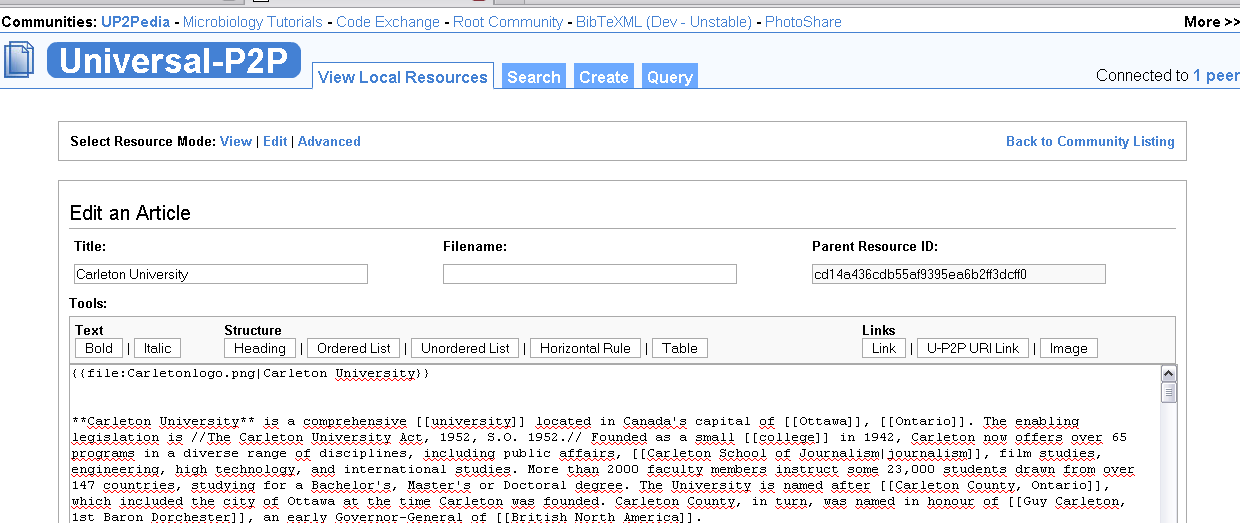
\includegraphics[scale=0.4]{screenshot.png}
\label{fig:screenshot}
\caption{A screenshot of the P2Pedia interface. The user is editing a page.}
\end{figure*}


The main difference with a traditional wiki is that as pages are downloaded to be viewed, they are also saved locally, and an edit creates a new version of the document, which is also stored locally. Therefore, as an article is edited, it may be ``forked" into multiple versions, and each peer is free to save and offer for download its preferred version. 

If a user searches for a page, different versions may be returned by different peers. The user may then use the versioning relationships between these versions, and trust indicators (detailed in section \ref{sec:trust}) about the documents and the peers, to decide which version to download. 

As multiple parallel versions may exist, users may also produce new versions by \emph{merging} several existing versions, selecting and reusing different parts of several \emph{parent} versions, and producing a single \emph{child} version. 

\subsection{Wiki Edition as an Application of File-sharing}

P2P File-sharing, mostly known as an application to share media files, can be applied to other types of content. Here, we show how the functionality of a distributed wiki can be mapped to an abstract model of file-sharing. We have used this mapping as a basis to implement P2Pedia on top of U-P2P, our file-sharing application \cite{UP2P2002, UP2PSemelsJournal2009, UP2P:201101TechReport}.

We first outline our model of file-sharing, implemented by U-P2P and more completely presented in \cite{UP2P:201101TechReport}. P2P file-sharing can be characterized as an application where peers, connected in a network, maintain a collection of \emph{documents} in a local repository. Peers may publish new documents to the repository, remove them, or copy (i.e. download) documents from other peers.

Peers can join or leave the network, and establish or drop connections with other peers. These operations define possible \emph{state changes} for the network. 

We then introduce the concept of a \emph{community}. A community is defined by a document \emph{schema} and a protocol (means for queries to reach peers). The schema is a set of attributes, and defines the type of documents that are shared in the community (music, video, or any other kind). consequently, it also defines which queries may be applied to these documents. 

This model can describe traditional file-sharing applications such as Limewire\footnote{official web site is http://www.limewire.com/, distribution currently suspended.} or Emule\footnote{http://www.emule-project.net/}. For example, Limewire can be defined as a community where MP3 music files are shared using the Gnutella 0.6 protocol with a TTL (time to live) of 7. The documents of this community are described by a file name, a binary ``payload", and a set of metadata properties, encoded in ``ID3 tags"\footnote{``ID3 tags" are data fields embedded into MP3 files, which identify the artist, song title, track number, etc.}. A peer may then communicate with all the peers reachable by a path of length of at most seven hops (seven edges in the connection graph), and can make queries on the file name, or on any of the ID3 metadata properties. 

An important feature of U-P2P is that community definitions can themselves be shared in the P2P network. This way, peers can create new such communities, and discover and download those created by others. A community description includes a document schema, which itself can be used as a guide for metadata-based searches.

We have further extended this model to include \emph{relations} between documents. Such relations are irrelevant to basic applications where ordinary media files are shared, but are useful for other types of documents, for example Wiki pages, which can be related by versioning relations and wikilinks.

For this purpose we have added a type of document attribute, called \emph{endpoints}, similar to web links. Endpoints rely on a naming scheme (i.e. a ``primary key" that unambiguously identifies any document), and represent a semantic link to that document, this semantics being carried by the attribute label. For example, our wiki pages refer to their \emph{parent} documents using such links. 

In addition to the semantics represented by the attribute label, an important difference with Web links is that endpoints, in a P2P file-sharing context, must point to \emph{any copy} of the target document, which may be replicated through the network. Looking up a document given its endpoint therefore means searching for all copies of the document by that unique name. The document naming scheme is therefore based on the document content rather than on an address. In practice, document identifiers in U-P2P are generated by a one-way hash function.

Graph queries can then be applied to the graph of documents (nodes), connected by endpoint attributes (edges) \cite{UP2P:201101TechReport}. 

Here, P2Pedia defines a community, where each shared file is a Wiki page. The document schema includes the page content (the wikitext), the versioning information, in the form of a multi-valued endpoint attribute to parent versions, and a number of wikilinks to other pages. The wiki engine is then simply a tool -- two small Javascript scripts -- provided as part of the community definition, for viewing and editing documents of the community.

The main functionality of the system is implemented by the standard file-sharing operations, namely publish, remove, query, and download. Searches for pages are implemented as file-sharing queries, and users download pages from other peers, just like any document in a file-sharing network. When peers edit pages, they create a new document, which links back to its parent documents using an endpoint attribute.

An endpoint attribute, as a link between two documents, can be viewed as a binary relation over the set of documents. The properties of the relations in P2Pedia (i.e. associated to the endpoint attributes of the P2Pedia schema) give a greater semantic interpretation to the graph queries made over  the P2Pedia document graph. In the next section, we define these semantic properties, and then show how appropriate queries over the graph of documents can be used to implement useful functionality for P2Pedia.

\subsection{Ancestry Relations, and the Semantics of Wikilinks}
\label{sec:ancestry}
The versioning process can be characterized by the properties of the \emph{parent} and \emph{child} binary relations between documents, and their respective transitive closures \emph{ancestor} and \emph{descendent}. 

The centralized collaboration model, implemented by traditional wikis, produces a linear versioning process, where the latest version is considered ``authoritative". If we consider each version of a page to be a separate document, a sequence of page versions is a set of documents, which all have the same page title, and the \emph{``child"} relation defines a total order over this set. This order is the order of the timestamps of the different versions. 

Wikilinks consequently have a clear semantics: a wikilink is defined by its \emph{label}, and points to the latest version of the page with that label for a title, i.e., within the set of page versions defined by that label, to the upper bound in the sense of the \emph{child} relation. 

In contrast, as we have mentioned above, the versioning process offered by our collaboration model produces a \emph{lattice} of versions for each page, where a given document version may have multiple \emph{children} versions (edits) and multiple \emph{parent} versions. Page titles and timestamps are then insufficient indicators of the version relationships between pages: the \emph{parent} and \emph{child} relation must be explicit within the pages, and define only a partial order over set of versions of a page with a given title. Figure \ref{fig:versioninglattice} shows this lattice versioning hierarchy compared with the sequential hierarchy produced by a centralized collaboration model (Figure \ref{fig:versioningsequence}). 

\begin{figure}[htb]
\centering
\subfigure[Versioning in a centralized Wiki: v3 is the ``current" version.]{
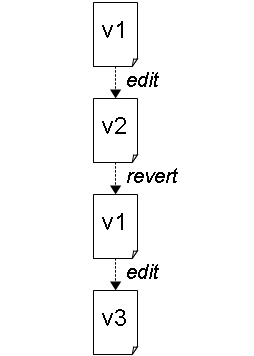
\includegraphics[scale=0.44]{versioning-sequence.png}
\label{fig:versioningsequence}
}
\subfigure[Versioning in P2Pedia: v5 and v6 are ``maximal" versions in the versioning lattice.]{
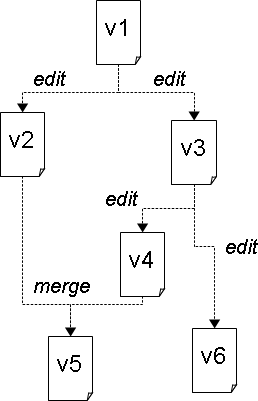
\includegraphics[scale=0.56]{versioning-lattice.png}
\label{fig:versioninglattice}
}
\caption{The different versioning processes available in a centralized and decentralized collaboration model produce different versioning hierarchy structures. Each figure shows an example hierarchy of versions for a single page.}
\end{figure}

Extending the notion of a wikilink to a set of page versions with a lattice structure is not trivial. In the linear case, there is always a single latest version, and we can therefore relate the document that the user originally linked to, with its unique last descendent, the current latest version. In the lattice case, there may be at any given time multiple ``latest" versions, and a user could intend to link to any one of these versions. Furthermore, from the originally linked version, there may be an entire tree of descendents, and any leaf of this tree would be a candidate to be the ``current version". 

This shows two requirements for wikilinks in this collaboration model. First, when creating a wikilink, a user should be able to explicitly choose any particular version of a page as the target. Secondly, the wikilink should link to multiple pages, i.e. it the link should return all the leaf-descendants of the originally linked document. 

Formally, this means that the binary relation defined by a wikilink defined within a document $A$, and originally pointing to document $B_0$, contains all pairs $(A, B_i)$ where $A$ is the document containing the link, and $B_i$ is a leaf-descendant of $B$.

The decentralized storage of our system further complicates the nature of the ancestry relation. As documents are copied through the network, the ``parent" links point to \emph{all copies} of the parent document version. The versioning process in Figure \ref{fig:versioninglattice}, combined with some downloads, could result in a distributed graph such as the one illustrated in Figure \ref{fig:versioning-deploy}. 

\begin{figure}[htb]
\centering
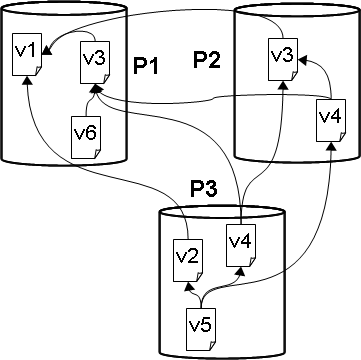
\includegraphics[scale=0.5]{doc-links-deploy.png}
\label{fig:versioning-deploy}
\caption{An example deployment of the document versions shown in Figure \ref{fig:versioninglattice}. The documents are distributed in three peers P1, P2, P3. The arrows represent ``parent" links between document versions.}
\end{figure}

A user may maintain a version that she consider ``authoritative", and if another peer has copied and edited this version, it is no longer a ``leaf" (maximal element) in the lattice of versions. Therefore in the above discussion, the leaves in the tree of descendents for a particular document must include the latest version stored by each peer, regardless of whether these version have been edited elsewhere.

In practice, this means that a wikilink is implemented as a search for all the descendents of the document that this link originally pointed to, and each peer returns its latest version. The search for the descendents of a page can be implemented by a generic U-P2P graph query that returns the transitive closure of the ``child" relation. The ``child" relation is not itself explicit in U-P2P, but its inverse relation ``parent" is implemented as an endpoint attribute, and can therefore be exploited by graph queries in U-P2P.

The class of graph queries supported by U-P2P \cite{UP2P:201101TechReport}, \emph{path queries}, are defined as follows. In the graph of interlinked documents, where documents are nodes and endpoint attributes are labeled edges, a path query can be defined by an input document $D$ and a sequence of labels $\pi = l_1,l_2 \dots, l_k$; an answer to this query is a document $A$ such that the edge labels on the path from $D$ to $A$ match $\pi$. The endpoint attributes are seen as directed edges, but queries can be defined for paths including the edges in both directions (i.e. both properties explicited by links and their implicit inverses can be queried, for example if the relation ``parent" is explicited by a link, then the relation ``child" can also be queried).

For P2Pedia we have extended this class of queries to include \emph{transitive closure} queries. This means that we can query for paths matching a particular sequence of symbols $l_1,l_2 \dots, l_k$, but also for paths matching the regular expression $l_0^{+}$.

P2Pedia supports queries for the transitive closure of ``parent" and its inverse, ``child", the latter being used to resolve wikilinks.

These queries return multiple documents, as do simple keyword searches. The user must then be assisted in choosing between them. For this purpose we introduce trust indicators, detailed in the next subsection. Note that in any search, the relevance to the query, as well as the visible ancestry of the versions, can be used to choose. However, in all cases, additional trust information may be useful. 

\subsection{Trust Indicators}
\label{sec:trust}

Traditional wikis often limit which users may contribute, or resolve conflicts as they occur, by attempting to determine (by a consensus, or by other decision processes), which single version of an document should be accepted. These principles can be described as centralized trust strategies, i.e. where the ``trustworthiness" of the contributors is a unique value determined by the overall system.

The collaboration model of U-P2P allows for multiple versions of the articles, and therefore it allows for decentralized trust strategies, i.e. strategies where each user may have its own trust level toward each peer (multiple-authority).

In P2Pedia, trust levels are not explicitly maintained within the system, but each time a user must choose a document between several versions offered by different peers, she is provided some indicators which may help her determine which peers and documents are the most trustworthy.

The indicators implemented in P2Pedia are listed hereafter.

\paragraph*{Peer Similarity} A measure of similarity between the collections of documents hosted by the two peers (i.e. the peer who is viewing the query results, and the peer who offers a particular result). This indicator is based on the assumption that users storing similar content (i.e. a high number of identical versions of documents) should trust one another more. The indicator given is the Jaccard similarity measure, i.e. the number of document ids in common divided by the total number of documents stored by the two peers.
\paragraph*{Network Distance} This indicator shows the distance between the peers in the connection graph. Assuming that peers connect to trusted acquaintances, and that trust has some level of transitivity, the network distance may help the peer decide on trust.
\paragraph*{Peer Popularity} The number of incoming connections to a remote peer. Again, if peers connect to trusted acquaintances, or decide to connect to peers that offer high quality content, then the indegree of a peer in the connection graph is a valuable indicator of general trustworthiness.
\paragraph*{Document Popularity} The total number of available sources for a given version of a document. This assumes that the replication of documents is a measure of their ``value". 
    
Note that for a peer to be deemed trustworthy according to the above indicators and to fully be able to use them for its own benefit, it must actively maintain its content (by keeping documents that it ``endorses" and deleting the others) and its neighborhood (by connecting to similar peers and disconnecting from those that it doesn't trust anymore).     

\section{Implementation}
\label{sec:implementation}
We briefly describe here the implementation of P2Pedia. It is important to note that as P2Pedia is conceptually defined with respect to an abstract model of file-sharing, its functionality could be implemented over other P2P architectures as well.

\subsection{U-P2P}

P2Pedia is implemented using the Universal Peer-to-Peer (U-P2P) framework \cite{UP2P2002, UP2PSemelsJournal2009, UP2P:201101TechReport}. 

The architecture of U-P2P is illustrated in Figure \ref{fig:TSarchitecture}.
\begin{figure}[htb]
	\centering
		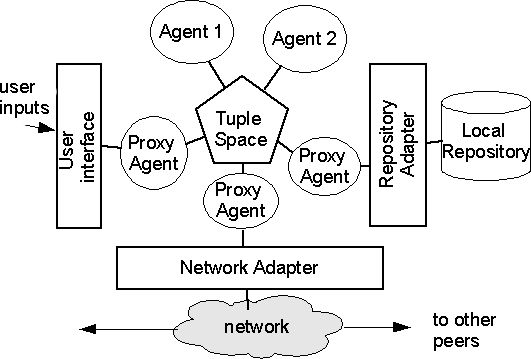
\includegraphics[scale=0.5]{U-P2Parchitecture.png}
	\caption{Architecture of U-P2P}
	\label{fig:TSarchitecture}
\end{figure}

The user interface of U-P2P is implemented with Java ServerPages and Servlets, and uses the Apache Tomcat Servlet Engine. Apache Xindice is used as the local XML database, and the Network Adapter uses a Java implementation of the Gnutella protocol. These three components are coordinated using a tuple space, which allows for asynchronous ad-hoc coordination, and seamless extension of the system functionality: additional components can be simply plugged into the tuple-space and make use of the file-sharing ``primitives" implemented by the main components. Graph query processing is implemented in this way, as described in the next section.

The Wiki functionality is implemented in Javascript using the JSCreole parser\footnote{http://jscreole.sf.net}.

\subsection{Implementation of Graph Queries}

As we have described in Section \ref{sec:ancestry}, U-P2P supports simple path queries over the graph of documents, and path queries using the transitive closure of an edge label.

We briefly describe here the implementation of path query answering in U-P2P. Our approach relies on multiple ``agents" generated on the fly from the query definition, and coordinated through the tuple space. For a path query defined by the path $\pi = l_1,l_2 \dots, l_k$ and the input document $D$, one agent is generated to process the sub-queries associated with each of the edge labels $l_i$. 

Starting from the input document $D$, the first ``agent"  must find all documents related to $D$ by an edge labelled $l_1$. Due to the asynchronicity of the P2P search protocol, the answers returned for this subquery arrive asynchronously in the tuple-space, and it is not known when the last answer has arrived (i.e. the termination can not be detected with certainty). The agent associated with $l_2$ asynchronously collects the answers from the previous subquery, and for each answer $d_{i}$ outputs a subquery to find documents related to $d_{i}$ by an edge labelled $l_2$. The answers to all of these subqueries are in turn collected by the next agent down the line, and in this way the different matching paths are explored in parallel to provide the answers to the overall path query.

The same processing can be slightly modified to answer a transitive closure query: a single agent is used, which recursively reuses the answers to its own subqueries. For a query to find the ancestors of some document $D_0$, i.e. documents related to $D_0$ by paths matching the transitive closure of the label ``parent", a single agent queries for the ``parent" documents of $D_0$, then for the parents of the answer documents, and this way recursively, until there are no more answers. Again, termination cannot be detected due to the asynchronicity of the search, so the searching agent remains active until the user runs a new query or closes the query answer page.

\subsection{Implementation of Trust Indicators}

The trust indicators in P2Pedia are either implemented by attaching additional meta-data to search response messages, or by extracting information included in the standard Gnutella protocol messages.
\paragraph*{Jaccard Index} When responding to a query the responding node includes a list of the documents it stores (only their identifiers), which the querying node can then use to calculate the Jaccard Index of the two sets. This increases the size of the messages and therefore constitutes a slight overhead.
\paragraph*{Network Distance} This value is determined by the querying node when receiving a search response by checking the Gnutella protocol ``hops" value on the incoming response. 
\paragraph*{Peer Popularity} The number of incoming connections to a node is included as meta-data in search responses. Note that this could be falsified by the node. Methods to infer the network topology by analyzing message hops should be explored to address this issue.
\paragraph*{Document Popularity} No additional meta-data is required for this indicator, as a querying node simply tracks the number of query hits it receives for a specific document. 

\subsection{On the Possibility of Deploying this System over a DHT}
As we have noted, this design could work on different insfrastructures. Most existing distributed wikis use DHTs to optimize the storage and access time of the documents. However, in our particular approach, the benefits of DHT would be much less important.
First, the principle of the system is that users freely maintain any version they like. Therefore storing all the versions according to a DHT protocol goes against this principle.

Secondly, we could consider using a DHT to optimize queries, following the idea of Emule, which uses the Kad DHT to support its query index. The problem here would be that the index would be huge, since the system is focused on text. The Emule approach is to index file names : for each work in a file name, place an index entry to the file in the appropriate DHT node. This implies that there exist perhaps at most 5 or 6 pointers for each file. In our case, as we support full-text search, we would need to index each word appearing in the document, and we would therefore need potentially hundreds of pointers to each file, which implies a very large index structure, that would imply major processing overhead.

\section{Evaluation and Validation}
\label{sec:evaluation}
The main novelty of our approach is the collaboration model supported by P2Pedia. The successful implementation and experimental deployment of P2Pedia shows the feasibility of using this collaboration model in a Wiki system.

We further outline here scenarios where this collaboration model may be more appropriate than the traditional, centralized collaboration model, and briefly discuss the technical performance of our system.

\subsection{Scenarios for this collaboration model}

In the collaboration model supported by P2Pedia, multiple versions of the documents are shared in a file-sharing network, and their versioning relations, as well as other trust indicators, are available for the users to choose thir preferred versions. Each user thus builds her own repository, storing a subset of the documents, filtered according to her interests and personal quality criteria.

As users may copy and edit documents, there is a simultaneous edition and selection process, which may lead to the most ``valuable" material to emerge.

We have identified several scenarios where this collaboration model could be a better alternative to the traditional centralized one. 

\subsubsection{Teaching Material} 
The Wikimedia foundation projects Wikibooks\footnote{http://wikibooks.org/} and Wikiversity\footnote{http://wikiversity.org/} are projects inspired by Wikipedia, where textbooks and other learning material are created collaboratively, following the centralized collaboration principles of traditional wikis. 

The benefit of these projects is that the learning material created this way is freely usable by instructors, and is assumed to reflect a form of consensus from the many contributors, which serves as quality assurance, as in Wikipedia. However, instructors rarely make use of a single source of learning material, and often prefer to combine various textbooks, selecting material according to their personal views on the topic. 

The collaboration model offered by P2Pedia would allow instructors to share their personal teaching material for a topic, partially reused from different sources, and possibly acknowledging these sources through versioning links. Trust indicators could indicate generally popular material, but also material from like-minded scholars.

\subsubsection{Collaborative Note Taking}
Following the principles outlined for general learning material, students could collaboratively take notes for their courses. Students are usually expected to take notes individually, in addition to reading textbooks and handouts. These notes are an opportunity for the student to personalize their learning material, by noting salient points, keeping a trace of oral explanations, and generally selecting material that they feel helps their understanding of the topic at hand.

Students may benefit from one another's lecture notes, and still want to study a version that is largely their own. We note that a stable and customized version of P2Pedia is to be deployed in the fall 2011 semester in several courses of Carleton University, as a note-taking tool. We intend to report on the success of this deployment in future work.

\subsubsection{Community-specific Knowledge Repositories}

In Wikipedia, the ``edit wars" that we hinted at in the introduction of this paper are an indication that even in the context of an encyclopedia, supposed to collect objective knowledge, a consensus may not always be found.

The alternative projects that we cited before, Citizendium and Scholarpedia, are not the only wiki-encyclopedias that have been created as a result of disagreements with Wikipedia policies. For example, a group of american conservatives, unhappy with the perceived political bias of Wikipedia, have created their own wiki-encyclopedia, called Conservapedia, with the purpose of describing the world according to their own political and religious views. This encyclopedia is several orders of magnitude smaller than Wikipedia, and focuses on political articles. 

Other examples can be cited, where alternative wiki-encyclopedias have been created to expand in great depth on narrow topics, such as religions or entertainment-related ``fandom" topics, such as the intricacies of a particular japanese Manga, or the fictional world of the Star Trek series. This results from the policy that only ``notable" topics can be covered by Wikipedia, as it is a general-purpose encyclopedia.

As a result, such spin-off encyclopedias only cover a small set of topics, and one can imagine that their users must combine that source of knowledge with others, for example Wikipedia: for example, for non-political and non-religious topics, such as the rules of cricket or the geography of Madagascar, Conservapedia users would probably turn to Wikipedia instead of copying that material to Conservapedia. 

\subsection{System Performance}

The technical characteristics of P2Pedia are essentially those of the underlying P2P file-sharing system. U-P2P uses the Gnutella protocol, which uses an unstructured, fully decentralized network. As such, P2P inherits the high reliability of Gnutella, but large networks may experience network congestion. However, research towards scalable P2P search is orthogonal to our main research goals.

The number and size of the shared documents in the network primarily affect (local) database access response times, but the database query times are generally negligible compared to network delays. As the number of versions of each article increases, the usability of the system may be degraded, as more effort is required from the users to sort and consider the different available versions. However, this is to be balanced with the effects of the trust indicators: larger numbers of peers and documents exhibit clearer and more statistically significant collective behavior. For example, the similarity of larger user repositories becomes more meaningful, and the replication of popular documents may reach significantly different counts from the background of unpopular documents. 

In our small experimental deployment, each document is only replicated once or a small number of times, which makes it difficult to visualize any clear tendencies. Furthermore, due to its small scale, the social network is entirely known to each participant, which makes notions of ``peer popularity" and ``network distance" irrelevant.  


\section{Conclusion}

The principles of file-sharing define basic operations for users to manage a local repository of documents, where they may import documents stored by others. By applying these principles to a wiki system, we have obtained an original system that supports a non-traditional collaboration model. In our wiki system, users create new documents, download them from others, and store them in their local repository just like any other files they could share in the underlying file-sharing application. The wiki functionality is simply an additional layer used by the web browser, whereby this web browser becomes an editing tool. We consider that the process of editing a document produces a new, separate document, related to the previous by a versioning relation. 

This versioning relation, materialized by a link, is simply an instance of a general \emph{document relation} concept, defined in the greater context of our file-sharing model. From the semantics of this ``parent" link, we can define further versioning relations, such as ``child", ``ancestor", ``descendent", which can be inferred from the ``parent" relation. This inference, here consists in using implicit inverse relations, and the notion of transitive closure. These notions can be obtained using graph query principles which are already defined for any type of links between documents.


In a sense, the underlying implementation of the queries does not need to know the semantics of the ``parent" relation, any more than the database needs to know that the documents being stored are wiki pages.

Ultimately, this application -- a full-fledged wiki engine -- is simply an application of general file-sharing principles, with the extra feature of document \emph{relations}. 

Similarly, the notions of trust that support the collaboration model, by allowing users to select the existing versions, are applicable to other file-sharing applications.

In future work, we intend to further customize our application P2Pedia, and deploy it as a note-taking tool, for several courses at Carleton University, and in an area high-school. This will be an opportunity to study the applicability of our approach, and the relevance of our proposed trust indicators.

We note that an online demo of P2Pedia is currently usable at the address http://inm-04.sce.carleton.ca:8080/up2p.

\bibliographystyle{IEEEtran}
\bibliography{rwj}

\end{document}
